% GNUPLOT: LaTeX picture with Postscript
\begingroup
\newcommand{\ft}[0]{\footnotesize}
  \makeatletter
  \providecommand\color[2][]{%
    \GenericError{(gnuplot) \space\space\space\@spaces}{%
      Package color not loaded in conjunction with
      terminal option `colourtext'%
    }{See the gnuplot documentation for explanation.%
    }{Either use 'blacktext' in gnuplot or load the package
      color.sty in LaTeX.}%
    \renewcommand\color[2][]{}%
  }%
  \providecommand\includegraphics[2][]{%
    \GenericError{(gnuplot) \space\space\space\@spaces}{%
      Package graphicx or graphics not loaded%
    }{See the gnuplot documentation for explanation.%
    }{The gnuplot epslatex terminal needs graphicx.sty or graphics.sty.}%
    \renewcommand\includegraphics[2][]{}%
  }%
  \providecommand\rotatebox[2]{#2}%
  \@ifundefined{ifGPcolor}{%
    \newif\ifGPcolor
    \GPcolortrue
  }{}%
  \@ifundefined{ifGPblacktext}{%
    \newif\ifGPblacktext
    \GPblacktextfalse
  }{}%
  % define a \g@addto@macro without @ in the name:
  \let\gplgaddtomacro\g@addto@macro
  % define empty templates for all commands taking text:
  \gdef\gplbacktext{}%
  \gdef\gplfronttext{}%
  \makeatother
  \ifGPblacktext
    % no textcolor at all
    \def\colorrgb#1{}%
    \def\colorgray#1{}%
  \else
    % gray or color?
    \ifGPcolor
      \def\colorrgb#1{\color[rgb]{#1}}%
      \def\colorgray#1{\color[gray]{#1}}%
      \expandafter\def\csname LTw\endcsname{\color{white}}%
      \expandafter\def\csname LTb\endcsname{\color{black}}%
      \expandafter\def\csname LTa\endcsname{\color{black}}%
      \expandafter\def\csname LT0\endcsname{\color[rgb]{1,0,0}}%
      \expandafter\def\csname LT1\endcsname{\color[rgb]{0,1,0}}%
      \expandafter\def\csname LT2\endcsname{\color[rgb]{0,0,1}}%
      \expandafter\def\csname LT3\endcsname{\color[rgb]{1,0,1}}%
      \expandafter\def\csname LT4\endcsname{\color[rgb]{0,1,1}}%
      \expandafter\def\csname LT5\endcsname{\color[rgb]{1,1,0}}%
      \expandafter\def\csname LT6\endcsname{\color[rgb]{0,0,0}}%
      \expandafter\def\csname LT7\endcsname{\color[rgb]{1,0.3,0}}%
      \expandafter\def\csname LT8\endcsname{\color[rgb]{0.5,0.5,0.5}}%
    \else
      % gray
      \def\colorrgb#1{\color{black}}%
      \def\colorgray#1{\color[gray]{#1}}%
      \expandafter\def\csname LTw\endcsname{\color{white}}%
      \expandafter\def\csname LTb\endcsname{\color{black}}%
      \expandafter\def\csname LTa\endcsname{\color{black}}%
      \expandafter\def\csname LT0\endcsname{\color{black}}%
      \expandafter\def\csname LT1\endcsname{\color{black}}%
      \expandafter\def\csname LT2\endcsname{\color{black}}%
      \expandafter\def\csname LT3\endcsname{\color{black}}%
      \expandafter\def\csname LT4\endcsname{\color{black}}%
      \expandafter\def\csname LT5\endcsname{\color{black}}%
      \expandafter\def\csname LT6\endcsname{\color{black}}%
      \expandafter\def\csname LT7\endcsname{\color{black}}%
      \expandafter\def\csname LT8\endcsname{\color{black}}%
    \fi
  \fi
  \setlength{\unitlength}{0.0500bp}%
  \begin{picture}(7936.00,6236.00)%
    \gplgaddtomacro\gplbacktext{%
      \colorrgb{0.50,0.50,0.50}%
      \put(594,751){\makebox(0,0)[r]{\strut{} 0}}%
      \colorrgb{0.50,0.50,0.50}%
      \put(594,1273){\makebox(0,0)[r]{\strut{} 5}}%
      \colorrgb{0.50,0.50,0.50}%
      \put(594,1795){\makebox(0,0)[r]{\strut{} 10}}%
      \colorrgb{0.50,0.50,0.50}%
      \put(594,2317){\makebox(0,0)[r]{\strut{} 15}}%
      \colorrgb{0.50,0.50,0.50}%
      \put(594,2839){\makebox(0,0)[r]{\strut{} 20}}%
      \colorrgb{0.50,0.50,0.50}%
      \put(594,3361){\makebox(0,0)[r]{\strut{} 25}}%
      \colorrgb{0.50,0.50,0.50}%
      \put(594,3883){\makebox(0,0)[r]{\strut{} 30}}%
      \colorrgb{0.50,0.50,0.50}%
      \put(594,4405){\makebox(0,0)[r]{\strut{} 35}}%
      \colorrgb{0.50,0.50,0.50}%
      \put(594,4927){\makebox(0,0)[r]{\strut{} 40}}%
      \colorrgb{0.50,0.50,0.50}%
      \put(594,5449){\makebox(0,0)[r]{\strut{} 45}}%
      \colorrgb{0.50,0.50,0.50}%
      \put(594,5971){\makebox(0,0)[r]{\strut{} 50}}%
      \colorrgb{0.50,0.50,0.50}%
      \put(773,484){\makebox(0,0){\strut{}1}}%
      \colorrgb{0.50,0.50,0.50}%
      \put(1067,484){\makebox(0,0){\strut{}2}}%
      \colorrgb{0.50,0.50,0.50}%
      \put(1361,484){\makebox(0,0){\strut{}3}}%
      \colorrgb{0.50,0.50,0.50}%
      \put(1656,484){\makebox(0,0){\strut{}4}}%
      \colorrgb{0.50,0.50,0.50}%
      \put(1950,484){\makebox(0,0){\strut{}5}}%
      \colorrgb{0.50,0.50,0.50}%
      \put(2244,484){\makebox(0,0){\strut{}6}}%
      \colorrgb{0.50,0.50,0.50}%
      \put(2538,484){\makebox(0,0){\strut{}7}}%
      \colorrgb{0.50,0.50,0.50}%
      \put(2832,484){\makebox(0,0){\strut{}8}}%
      \colorrgb{0.50,0.50,0.50}%
      \put(3126,484){\makebox(0,0){\strut{}9}}%
      \colorrgb{0.50,0.50,0.50}%
      \put(3421,484){\makebox(0,0){\strut{}10}}%
      \colorrgb{0.50,0.50,0.50}%
      \put(3715,484){\makebox(0,0){\strut{}11}}%
      \colorrgb{0.50,0.50,0.50}%
      \put(4009,484){\makebox(0,0){\strut{}12}}%
      \colorrgb{0.50,0.50,0.50}%
      \put(4303,484){\makebox(0,0){\strut{}13}}%
      \colorrgb{0.50,0.50,0.50}%
      \put(4597,484){\makebox(0,0){\strut{}14}}%
      \colorrgb{0.50,0.50,0.50}%
      \put(4891,484){\makebox(0,0){\strut{}15}}%
      \colorrgb{0.50,0.50,0.50}%
      \put(5186,484){\makebox(0,0){\strut{}16}}%
      \colorrgb{0.50,0.50,0.50}%
      \put(5480,484){\makebox(0,0){\strut{}17}}%
      \colorrgb{0.50,0.50,0.50}%
      \put(5774,484){\makebox(0,0){\strut{}18}}%
      \colorrgb{0.50,0.50,0.50}%
      \put(6068,484){\makebox(0,0){\strut{}19}}%
      \colorrgb{0.50,0.50,0.50}%
      \put(6362,484){\makebox(0,0){\strut{}20}}%
      \colorrgb{0.50,0.50,0.50}%
      \put(6656,484){\makebox(0,0){\strut{}21}}%
      \colorrgb{0.50,0.50,0.50}%
      \put(6951,484){\makebox(0,0){\strut{}22}}%
      \colorrgb{0.50,0.50,0.50}%
      \put(7245,484){\makebox(0,0){\strut{}23}}%
      \colorrgb{0.50,0.50,0.50}%
      \put(7539,484){\makebox(0,0){\strut{}24}}%
      \csname LTb\endcsname%
      \put(220,3361){\rotatebox{-270}{\makebox(0,0){\strut{}Przyspieszenie S}}}%
      \put(4156,154){\makebox(0,0){\strut{}Liczba wątków}}%
    }%
    \gplgaddtomacro\gplfronttext{%
      \csname LTb\endcsname%
      \put(2225,5798){\makebox(0,0)[r]{\strut{}OMP parfor}}%
      \csname LTb\endcsname%
      \put(2225,5578){\makebox(0,0)[r]{\strut{}MKL DGEMM}}%
      \csname LTb\endcsname%
      \put(2225,5358){\makebox(0,0)[r]{\strut{}Naiwny}}%
    }%
    \gplbacktext
    \put(0,0){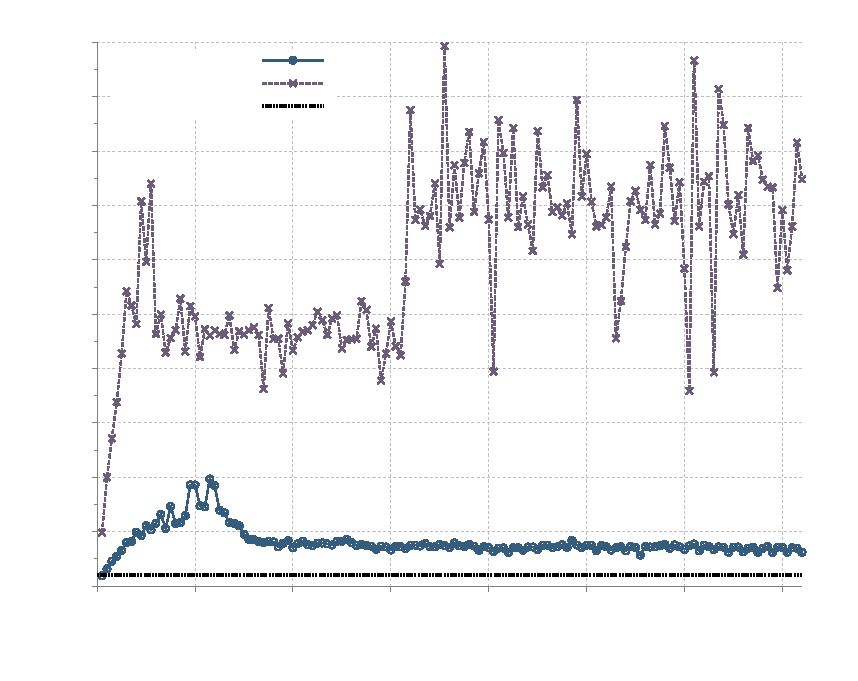
\includegraphics{mono}}%
    \gplfronttext
  \end{picture}%
\endgroup
